% -*- root: diplomarbeit.tex -*-
\section{Tracking Learning Detection - TLD}
	Die originale Implementation von TLD erfolgte in Matlab. Teil dieser Arbeit ist eine Adaption in C++. Zum Verständnis der einzelnen Komponenten und für die Darstellung der Arbeitsweise wird in diesem Kapitel der Algorithmus im Detail vorgestellt und theoretisch betrachtet.

	\subsection{Tracking}
	Die Tracker-Komponente hat im Wesentlichen die Aufgabe die Bewegung eines Objekts $o$ zu schätzen, wobei typischerweise die Annahme besteht, dass das Objekt in einer Bildsequenz sichtbar ist. Es gibt in der Praxis eine Reihe von Ansätzen, die sich hinsichtlich der Repräsentation des Objekts, zum Beispiel als Punkte, Kontouren, Modelle oder optischer Fluss, als auch der algorithmischen Verarbeitung unterscheiden.

	In dieser Arbeit wird, wie im grundlegenden TLD-Ansatz, der MediaFlow- Tracker \cite{MFT} implentiert. Der Grundgedanken basiert auf der\textit{ forward-backward consistency assumption}, die besagt, dass erfolgreiches Verfolgen unabhängig von der Richtung des Zeitflusses sein sollte. Als erstes wird eine Menge von gleichverteilten Punkten, definiert durch die BoundingBox, in einem Bild $t$ erzeugt. Im nächsten Schritt erfolgt die \textit{forward} Bestimmung des optischen Flusses mittels Lucas-Kanade-Algorithmus \cite{OPT} im Bild $t+1$. Die Punktemenge, die dadurch ermittelt wurde, wird nun \textit{backward} für die Bestimmung des optischen Flusses im Bild $t$ genutzt. Die Informationen aus beiden Lucas-Kanade-Berechnungen werden zur Bestimmung es \textit{Forward-Backward Errors (FB)} um fehlerhafte Punkte zu filtern. Die verbliebenen Punkte bestimmen die Transformation der BoundingBox. Abbildung \ref{fig:MFT} verdeutlicht das Prinzip.

	\begin{figure}
	\centering{}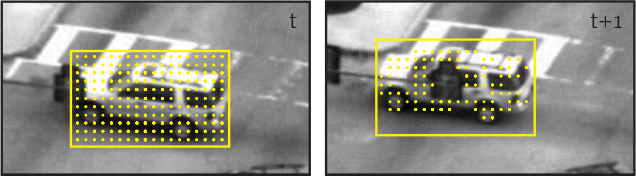
\includegraphics[scale=0.7]{../pictures/MediaFlow_0.png}\caption[Arbeitsweise des Median Flow Trackers]{Arbeitsprinzip des Median Flow Trackers. Alle Punkte, die sowohl in $t$ als auch in $t+1$ vorhanden sind, werden als Grundlage für die Berechnung der BoundingBox gentutzt. (Quelle: \cite{MFT})\label{fig:MFT} }
	\end{figure}

	\subsubsection{Der optischen Flusses und der Lucas-Kanade-Algorithmus}
	Die Berechnung des optischen Flusses entspricht im Wesentlichen der folgenden Aufgabe: Finde den Punkt $x$ aus Bild $I_{0}$ im Bild $I_{1}$ beziehnugsweise in einer Sequenz von Bildern $I_{1},..,I_{n}$. Lucas und Kanade gehen zur Berechnung von drei Annahmen aus.

	\begin{enumerate}
	\item \textit{Brightness constancy.} Das Erscheinungsbild eines Pixel eines Objekts in einer Sequenz bleibt unverändert. Für Grauwertbilder bedeutet das, dass die Helligkeit (\textit{brightness}) eines Pixels Konstant bleibt, wenn dieser von Bild zu Bild verfolgt wird.
	
	\begin{equation}
	I_{0}(x)=I_{1}(x+d)
	\end{equation}

	\item \textit{Temporal persistence. }Die Positionsänderung eines Objekts in einer Bildsequenz ist gering. Das bedeutet, dass die Geschwindigkeitsvectoren klein sind. Diese können im zweidimensionalen Fall mit der folgenden partiellen Ableitung berechnet werden:
	
	\begin{equation} I_{x}u+I_{y}v+I_{t}=0, \end{equation}
	mit $u,v$ als die gesuchten Geschwindigkeitsvectoren für die Koordinatenänderung für $x$ und $y$ im Bild $I$ und $I_{t}$ als zeitliche Änderung zwischen den Bildern. Allerdings ist diese Gleichung für einzelne Pixel nicht eindeutig lösbar, da durch die gesuchten Vectoren $u,v$ zwei Unbekannte existieren. Der Ergebnisraum wäre somit ein Linie und kein einzelner Punkt. Dieses Problem wird durch die dritte Annahme behandelt.

	\item \textit{Spatial coherence.} Punkte in einer Nachbarschaft gehören zur einer Oberfläche und verhalten sich gleich. Der gesuchte Punkt bildet das Zentrum eines $5\times5$ Pixel großen Ausschnitts.
	%\footnote{Auch andere Größen, wie $3\times3$ oder $7\times7$, sind denkbar. Allerdings wird die dritte Annahme mit steigender Ausschnittsgrößen nich mehr erfüllt%}. 
	Mit Hilfe der Nachbarpunkte, deren Geschwindigkeit nach Annahme gleich ist, kann das folgende Gleichungssystem mit 25 Gleichungen erzeugt werden:

	\begin{equation}
	\left[\begin{array}{cc}
	I_{x}(p_{1}) & I_{y}(p_{1})\\
	I_{x}(p_{2}) & I_{y}(p_{2})\\
	\vdots & \vdots\\
	I_{x}(p_{25}) & I_{y}(p_{25})
	\end{array}\right]\left[\begin{array}{c}
	u\\
	v
	\end{array}\right]=-\left[\begin{array}{c}
	I_{t}(p_{1})\\
	I_{t}(p_{2})\\
	\vdots\\
	I_{t}(p_{25})
	\end{array}\right].
	\end{equation}
	\end{enumerate}
	Mittels Methode der kleines Quadrate kann die Lösung des Gleichungssystems minimiert werden. Für weitere Details zur Implementierung in \textit{OpenCV}
	siehe \cite{OCV}.
	
	\subsubsection{FB, NCC und Median Flow Tracker}
	Sei $S=(I_{t},I_{t+1},..,I_{t+k})$ eine Bildsequenz und sei $x_{t}$ ein Punkt zur Zeit $t$. Unter Verwendung eines beliebigen Trackers wird $x$ in $k$ Bildern aus $S$ verfolgt. Die erzeugte Trajektorie ist $T_{f}^{k}=(x_{t},x_{t+1},...,x_{t+k})$, mit $f$ für \textit{forward} der Länge $k$. Ziel ist es nun die Gültigkeit von $T_{f}^{k}$zu bestimmen. Hierzu wird der Punkt $x_{t+k}$\textit{backward} zum ersten Bild $I_{t}$ verfolgt. Der resultierende Trajektorie ist $T_{b}^{k}=(\hat{x}_{t},\hat{x}_{t+1},...,\hat{x}_{t+k})$, mit $b$ für \textit{backward} und $\hat{x}_{t+1}=x_{t+1}$. Der Fehler zwischen beiden Trajektorien ist definiert als $FB=distance(T_{f}^{k},T_{b}^{k})$, mit dem euklidischen Abstand zwischen dem initialen Punkt $x_{t}$ von $T_{f}^{k}$ und dem letzten Punkt $\hat{x}_{t}$ von $T_{b}^{k}$, also $distance(T_{f}^{k},T_{b}^{k})=||x_{t}-\hat{x}_{t}||$.

	Abbildung \ref{fig:Prinzip-des-Media} verdeutlicht das Erkennen von Tracking-Fehlern. Im linken Bild ist Punkt 1 in beiden Bildern sichtbar, also sind \textit{forward}- und \textit{backward}-Trajektorien identisch und der Tracker kann ihn korrekt verfolgen. Punkt 2 hingegen ist im rechten Bild verdeckt, was zu einer Bestimmung eines falschen Punktes führt. In der Konsequenz unterscheiden sich \textit{forward}- und \textit{backward}-Trajektorie und durch die Berechnung des \textit{Forward-Backward Errors} kann dieser Fehler leicht erkannt und behandelt werden.

	\begin{figure}
	\begin{centering}
	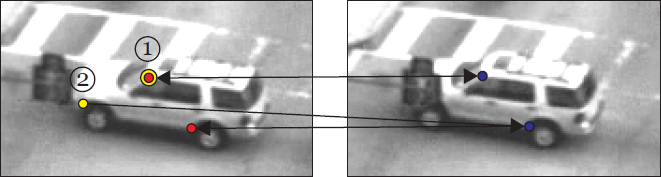
\includegraphics[scale=0.7]{../pictures/MediaFlow.png}
	\par\end{centering}

	\caption[Erkennen von Tracking-Fehlern]{Erkennen von Tracking-Fehlern. Die forward-backward-Trajektorien von Punkt 1 stimmen überein, da dieser in beiden Bildern existiert. Für Punkt 2 weichen sie jedoch segnifikant ab, weil dieser im zweiten Bild verdeckt ist. (Quelle: \cite{MFT})\label{fig:Prinzip-des-Media}}
	\end{figure}

	Neben dem Forward-Backward Error wird von Kalal et al.\cite{TLD}ein weiteres Messverfahren implementiert, der die Leistungsfähigkeit des Trackers signifikant verbessert\cite{MFT}. Mittel hierfür ist der \textit{Normalized Crorrelation Cefficient (NCC)}. % \begin{comment} HIER NOCH DIE FORMEL??? \end{comment}
	Es werden nicht nur die gesuchten Pixel, sondern auch deren umgebeneNachbarn analysiert. Dazu werden $10\times10$ Pixel große Patches, ausgehend vom verfolgten Punkt, generiert und mit einem ebenso erzeugten Patch des möglicherweise entsprechenden Punktes auf Ähnlichkeit untersucht. Sind sich beide ähnlich genug, dann wird der gefundene Punkt als valide angesehen.

	Der implentierte \textit{Median Flow Tracker} wendet das \textit{Forward-BackwardError}-Prinzip in Verbindung mit der Berechnung des \textit{NCC} entsprechend \cite{key-5} an. In Alg.\ref{alg:tracking} ist der Algorithmus skizziert. Als Eingabe dienen das letzte Bild $I$ mit der dazugehörige BoundingBox$B_{I}$ sowie das Folgebild $J$. Zur Berechnung der gültigen Punkte werden die Mediane des FB $median_{fb}$und des \textit{NCC} $median_{ncc}$genutzt. Hierbei werden die Punkte verworfen, deren FB größer als $median_{fb}$ und deren Ähnlichkeitswert kleiner als $median_{ncc}$ ist. Falls $median_{fb}$ größer als ein Treshold $th_{fb}$ ist, wird das Ergebnis durch LK als falsch interprätiert und verworfen. Die restlichen Punkte und $B_{I}$ dienen zur Berechnug der nächsten BoundingBox $B_{J}$. Hierzu wird der Median der Abstände aller Punkte in $I$ und in $J$ berechnet die Änderungen als Grundlage für die Verschiebnung in x- und y-Richtung genutzt. Die Skalierung von $B_{J}$ ist die relative
	Änderung der Abstände.

	\begin{algorithm}[h]
	\textbf{Input} $I,J,B_{I}$ \\
	\textbf{Output} $B_{J}$\\
	Generiere Punkte $p_{1},\ldots,p_{n}$ mittels $B_{I}$\\
	\textbf{for all} $p_{i}$\\
	\textbf{do}\\
	\ \ $p'_{i}=LK(p_{i})$\\
	\ \ $p''_{i}=LK(p'_{i})$\\
	\ \ $fb_{i}=|p_{i}-p''_{i}|$\\
	\ \ $ncc_{i}=NCC(p_{i},p'_{i})$\\
	\textbf{end}\\
	\ \ $median_{fb}=median(fb_{1}\ldots fb_{n})$\\
	\textbf{if} $median_{fb}>th{}_{fb}$ \textbf{then}\\
	\ \ $B_{J}=\emptyset$\\
	\textbf{else}\\
	\ \ $median_{ncc}=median(ncc_{1}\dots ncc_{n})$\\
	\ \ $q=validePoints(p,median_{fb},median_{ncc})$\\
	\ \ $B_{J}=calcBoundingBox(q,B_{I})$\\
	\textbf{end}
	\caption{Tracking}
	\label{alg:tracking}
	\end{algorithm}

	\newpage{}

	\subsection{Detection}
	Wenn das verfolgte Objekt den Bildbereich verlässt oder durch andere Objekte verborgen wird, kann die Tracker-Komponente nicht weiterarbeiten. Das Model zur Berechnung der Trajektorie fehlt. Aus diesem Grund ist eine Detection-Komponente erforderlich, die versucht das Objekt im Bild zu finden. Typischerweise ist diese Aufgabe recht aufwendig und die Umsetzung stark von der Art der Repräsentation des Ojekt-Modells abhängig.

	In dieser Arbeit wird wie in \cite{TLD} beschrieben, ein kaskadierender Detector implementiert. Grundlage für das Durchsuchen eines Bildes ist die \textit{Sliding-Window}-Methode \cite{key-6}. Hierbei wird ein Gitter definiert, das über das Bild gelegt wird. Jedes Feld des Gitters ist ein Ausschnitt (\textit{window}) des Bildes und wird einzeln durch mehrere Klassifizierer bewertet. Sollte ein solches Teilbild am Ende der Kaskade nicht verworfen worden sein, ist es ein Kandidat für das gesuchte Objekt. Die Größe des Gitters wird durchdie initiale BoundingBox bestimmt, da die einzelnen Felder Skalierungen dieser sind. 

	Die Kaskade des Detectors besteht aus drei Teilen, dem Varianzfilter, dem \textit{Ensemble-Classifier} und als letzte Instanz der \textit{NearestNeigbour-Classifier}, die im folgenden einzeln vorgestellt werden. Dabei ist der Grundgedanke, dass ein gesuchtes Objekt komplexer als der Bildhintergrund ist. Jeder Teil hat die Aufgabe, die \textit{windows} zu Klassifizieren und entweder zu verwerfen, da sie nicht dem gesuchten Objekt entsprechen können, oder an den nächsten Klassifizierer weiterzureichen, wenn keine eindeutig negative Aussage getroffen werden kann. Nach einer kompletten Abarbeitung des Gitters werden die übrig gebliebenen Kandidaten mittels Cluster-Verfahren gruppiert. Als Kriterium dient der Grad der Überlappung der einzelnen \textit{windows.} Aus jedem Cluster wird abschließend eine gemittelte BoundingBox berechnet, die ein mögliches gefundenes Objekt repräsentiert. Im Gegensatz zu vielen anderen Detector-Ansätzen, benötigen diese Implementation keine offline-Trainingsdaten. Die Lernkomponente, bestehend aus Ensemble-Classifier und Nearest-Neighbour-Classifier, wird mit der ersten BoundingBox initialisiert. Alle weiteren Trainingsbeispiele werden mit Hilfe des Trackers und der P-N Learning-Komponente erzeugt. Genaueres folgt im Punkt Maschinelles Lernen.

	\begin{algorithm}[H]
	\vspace{0.5cm}
	% Anpassen der Darstellung für c-style
	\SetStartEndCondition{ (}{)}{)}\SetAlgoBlockMarkers{}{\}}%
	\SetKwProg{Fn}{}{\{}{}\SetKwFunction{FRecurs}{void FnRecursive}%
	\SetKwFor{For}{for}{\{}{}%
	\SetKwIF{If}{ElseIf}{Else}{if}{\{}{elif}{else\{}{}%
	\SetKwFor{While}{while}{\{}{}%
	\SetKwRepeat{Repeat}{repeat\{}{until}%
	\AlgoDisplayBlockMarkers\SetAlgoNoLine%

	\KwData{Input}
	\KwResult{OUTPUT }
	initialization\;
	\While{not at end of this document}{
	read current\;
	\eIf{understand}{
	go to next section\;
	current section becomes this one\;
	}{
	go back to the beginning of current section\;
	}
	}
	\caption{Detection}
	\end{algorithm}

	\subsubsection{Objekt-Modell}
	Die Modellierung des Objekts und dessen Umgebung erfolgt in einer speziellen Datenstruktur
	\begin{equation}
	M=\{p_{1}^{+},p_{2}^{+},\dots,p_{m}^{+},p_{1}^{-},p_{2}^{-},\dots,p_{n}^{-}\}.
	\end{equation}
	Die Patches $p^{+}$bilden hierbei die positiven Beispiele, die das Objekt identifizieren ($p_{1}^{+}$bildet hierbei das initiale Objekt, das durch die Definition der BoundingBox erzeugt wurde). Die $p^{-}$ sind eine Sammlung negativer Beispiele, die aus der Umgebung der BoundingBox ermittelt werden. Während der Ausführung des Algorithmus' wird das Objekt-Modell stetig mit neuen positiven und negativen Beispielen erweitert. Die Strategie wird im Kapitel Maschinelles Lernen näher beschrieben.

	\subsubsection{Sliding-Window}
	Aus der initialen \textit{BoundingBox} werden alle möglichen Skalierungen und Verschiebungen dieser Box generiert. Damit wird das gesamte Bild mit den verschiedenen Größen und Positionen, die das Objekt annehmen kann, überdeckt. Für die Erzeugung des so entstehenden Gitters werden die folgenden Parameter genutzt: Skalierungs-Schritt$=1.2$, horizontale Verschiebung $=10\%$ der Breite, vertikale Verschiebung $=10\%$ der Höhe, Mindestgröße einer Box $=20\times20$ Pixel. Für ein Bild mit einer Auflösung von $640\times480$ Pixel ergeben sich bis zu $200.000$ \textit{BoundingBoxes}. Die tatsächliche Anzahl ist allerdings von der initialen BoundingBox abhängig. Für Geschwindigkeitsverbesserungen, kann die Mindestgröße einer Box auf $40\times40$ Pixel erhöht werden, wodurch nur noch bis zu $50.000$ BoundingBoxes erzeugt werden. Die Resultate des Detectors werden dadurch nicht signifikant schlechter.

	\subsubsection{Varianzfilter}
	Die erste Stufe des kaskadierenden Classifier bildet der Varianzfilter. Dieser vergleicht alle Patches, die durch das Grid gegeben sind, und verwirft die, deren Varianz kleiner als die Varianz des gesuchten Objekts ist. Dadurch können uniforme Regionen wie Hintergründe (Himmel, Wände etc.) schnell erkannt und verworfen werden um so den Suchraum zu verkleinern.

	Die Berechnung der Varianz kann sehr schnell mittels integralen Bildern (\textit{integral images}) erfolgen \cite{key-6}. Dabei handelt es sich um eine spezielle Datenstruktur, die eine einfache und schnelle Summierung von Pixelwerten beliebiger Regionen in einem Bild in $O(1)$ erlaubt. Zur Veranschaulichung siehe Abb. \ref{integralImg}. Für eine Bild $i$ der Größe $w,h$ ist das integrale Bild $ii$ eine Struktur der Größe $w+1,h+1$, wobei die erste Zeile und die erste Spalte jeweils mit $0$ gefüllt sind. Alle anderen Pixelwerte entsprechen der Summe der Pixel links und über dem Pixel, addiert mit dem eigenen Wert.

	\begin{figure}[h]
	\centering{}%
	\begin{tabular}{|c|c|c|}
	\hline
	4 & 3 & 1
	\tabularnewline
	\hline
	\hline
	2 & 4 & 3
	\tabularnewline
	\hline
	8 & 10 & 4
	\tabularnewline
	\hline
	\end{tabular} %
	\begin{tabular}{|c|c|c|c|}
	\hline
	0 & 0 & 0 & 0
	\tabularnewline
	\hline
	\hline
	0 & 4 & 7 & 8\tabularnewline
	\hline
	0 & 6 & 19 & 30
	\tabularnewline
	\hline
	0 & 14 & 43 & 57
	\tabularnewline
	\hline
	\end{tabular}\caption{Darstellung der Pixelwerte eines $3\times3$ Bildes (links) und des
	dazugehörigen integralen $4\times4$ Bildes (rechts).}
	\label{integralImg}
	\end{figure}

	Die Berechnung kann in linearer Zeit mittels einmaliger Iteration über das Bild durchgeführt werden.

	$$ ii(x,y)=\underset{x'\leq x}{\sum}\underset{y'\leq y}{\sum}i(x',y'). $$
	Der Vorteil der integralen Bilder liegt nun in der schnelle Berechnung von Pixelwerten innherhalb rechteckiger Teilbildern, die dann für weitere Berechnungen oder als Vergleichskriterium dienen. Die Summe der Pixel für ein Quadrat $ABCD$, siehe Abb. \ref{Subwindow}, kann mit Hilfe von vier Array-Referenzen berechnet werden. Da $D$ die Summe aller verherigen Pixel ist, müssen die Werte von $B$ und $C$ subtrahiert werden, weil sie nicht Teil von $ABCD$ sind. Da allerdings der Wert von $A$ dadurch zweimal abgezogen wurde, muss $A$ abschließend wieder dazuaddiert werden. Daraus ergibt sich die Formel $$ABCD=D+A-C-B$$ für die Summe der Pixelwerte eines Teilbildes $ABCD$.

	\begin{figure}
	\centering{}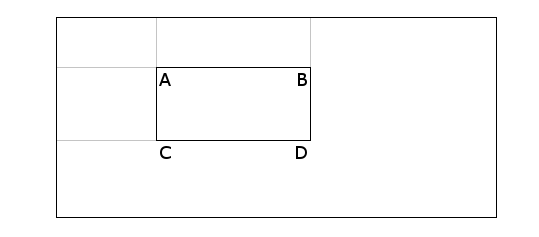
\includegraphics[scale=0.7]{../pictures/IntegralImage.png}\caption{Teilbild $ABCD$}
	\label{Subwindow}
	\end{figure}

	Neben dem integralen Bild können auch weitere Strukturen, wie das quadratische integrale Bild $ii^{2}$ auf ähnliche Weise berechnet werden. In der Implementierung wird das auch getan, um die Varianz durch $var(p)=ii^{2}(p)-i(p)^{2}$ zu berechnen. WELCHE VORTEILE HAT DAS GENAU??? HIER MUSS NOCH WAS ZUR ERKLÄRUNG HIN!!! 

	Auf die beschriebene Weise werden nun die Varianzen der einzelnen möglichen Objekte, die durch das Grid definiert sind, mit dem Varianzwert des aktuellen BoundingBox verglichen, und bei einem geringeren Wert verworfen. Alle übrig gebliebenen Boxen werden im folgendenen \textit{Essemble Classifier} verarbeitet.

	\subsubsection{Ensemble-Classifier}
	Wurde ein Patch nicht durch den Varianzfilter verworfen, gelangt er zur zweiten Stufe der Kaskade, dem EnsembleClassifier. Dieser besteht aus einer Menge so genannter Base-Classifier, die einzeln eine Bewertung zu dem übergebenen Patch abgeben. Aus deren Ergebnisse wird ein Mittelwert gebildet, der dann die Bewertung des \textit{Ensemble-Classifiers} ist.

	\paragraph{Random Ferns}
	Grundlage des Klassifizierers ist die in XXX vorgestellte \textit{random fern classification}-Methode. Das Ensemble der Base-Classifier besteht aus $n$ Ferns, von denen jeder unabhängig den Patch $I$ bewertet. Dafür vollzieht jeder Fern $i$ eine Anzahl binärer Pixelvergleiche zweier zufällig gewählter Pixel im Patch, mit

	\begin{equation}
	f_{i}=\begin{cases}
	0, & I(d_{i,1})<I(d_{i,2})\\
	1, & sonst
	\end{cases}
	\end{equation}

	Aus den Vergleichen der einzelnen Features, also zweier Pixelwerte, wird ein binären Code $x$ erzeugt. Der entsprechende dezimale Wert ist wiederum Index für ein Feld von A-Posteriori-Wahrscheinlichkeiten $P_{i}(y|x)$, mit $y\in{0,1}$. Aus allen berechneten Wahrscheinlichkeiten jedes Ferns wird dann ein Mittelwert berechnet und falls diese kleiner als $0.5$ ist, wird der Patch verworfen.

	Die zufällig gewählten Features werden bei der Initialisierung des \textit{Ensemble-Classifiers} berechnet und bestehen während der Laufzeit des Programms unverändert. Da der Vergleich zweier Pixel ein sehr schwaches Unterscheidungskriterium ist, muss eine große Anzahl von Features für jeden Fern erzeugt werden. Anders ausgedrückt sollte das Feld der A-Posteriori-Wahrscheinlichkeiten möglichst viele Einträge haben. Für ein $P_{i}$ ergibt sich $2^{d}$ als Feldgröße, wobei $d$ die Anzahl der Features für ein $i$ist. In der Implementierung führt jeder Fern $13$ Pixelvergleiche durch, was in $8.192$ möglichen Codes resultiert. Die A-Posteriori-Wahrscheinlichkeit wird durch $P_{i}(y|x)=\frac{\#p}{\#p+\#n}$ berechnet, mit $\#p$ als Anzahl der positiven und $\#n$ als Anzahl der negativen Bewertungen eines Ferns $i$ für den Code $x$ ist.

	\begin{figure}[H]
	\begin{centering}
	\includegraphics[scale=0.5]{../pictures/EnsembleBeispiel.jpg}
	\par\end{centering}
	\caption{Prinzipielle Arbeitsweise der \textit{Base-Classifier}.}
	\label{EnCl}
	\end{figure}

	Abbildung \ref{EnCl} verdeutlich das Prinzip. Das Ensemble besteht aus drei Ferns mit jeweils vier Feature. Die in jedem Kästchen dargestellte Punkte stellen die Pixel im Bild da und werden jeweils paarweise verglichen. Pro Kästchen also der Pixelwert des schwarzer mit dem des weißen Punktes. Die vier binären Vergleiche pro Fern resultiert in einem binären Code, für Fern 1 ist dieser beispielsweise $1100$. Dieser Code wird nun dezimal interprätiert und dient als Index im\textit{ Posterior}-Array, im genannten Beispiel also $1100_{2}=12_{10}$ und damit $P_{1}[12]=0.6$.

	% \begin{comment}
	% ERKLÄRUNG ZUR FUNKTIONSWEISE DES FERNCLASSIFIER (Was sind Ferns? Die
	% Idee? Binäre KLassifizierung eines Bildes mittels ``Maske'' - da
	% sehr schwach muss es viele Klassifizierer geben (Das ist auch besser,
	% siehe Quelle {[}bla{]}), Ähnlichkeiten zu RandomForest, warum ist
	% Fern besser, Wie wurde implementiert, Initialisierung, Update etc...

	% Initialisierung: 10 pos (die besten, also conf > 0.5) und 100 neg
	% Beispiele (willkürlich)

	% Anfangs werden die Patches mit einem Gaußfilter (Standardabweichung von 3 Pixel)
	% \end{comment}
	\subsubsection{Template-Matching und Nearest-Neighbour-Classifier}

	\paragraph{Template-Matching}
	Die letzte Stufe des Klassifizierers ist ein Nearest-Neighbour-Classifier, der mittels Template-Matching die verbliebenen Patches klassifiziert. Bei diesem Verfahren wird der gesuchte Patch (das Template) $T$ direkt in einem Bild $I$ gesucht, indem es über dieses geschoben und mittels einer Matching-Methode, in dieser Implementation durch Berechnung des (normalisierten) Korrelations-Koeffizienten, verglichen wird. Dabei wird der relative Mittelwert von $T$ mit dem relativen Mittelwert von $I$ verglichen. Das Ergebnis ist ein Wert zwischen $1$(perfekter Match) und $-1$(perfekter Missmatch). $0$ bedeutet, dass zwischen $T$ und $I$ keine Korrelation exisitert. Da es sich hierbei um eine sehr konservative und rechenintensive Vergleichsmethode handelt, bildet sie den Abschluss der Kaskade.

	Der Korrelations-Koeffizient wird wie folgt berechnet:

	\begin{equation}
	CC(x,y)=\underset{x',y'}{\sum}[T'(x',y')\times I'(x+x',y+y')]^{2}
	\end{equation}


	\begin{equation}
	T'(x',y')=T(x',y')-\frac{1}{(w\times h)\underset{x'',y''}{\sum}T(x'',y'')}
	\end{equation}


	\begin{equation}
	I'(x+x',y+y')=I(x+x',y+y')-\frac{1}{(w\times h)\underset{x'',y''}{\sum}I(x+x'',y+y'')}
	\end{equation}


	Um Fehler zu reduzieren, die durch eine unterschiedliche Beleutung
	des Templates $T$ und des Bildes $I$ entstehen können und damit
	das Ergebnis verfälschen, wir der Koeffizient normalisiert. Zusätzlich
	wird das Ergebnis umgerechnet, das Ergebnis im Intervall $[0..1]$
	liegt.

	\begin{equation}
	S(x,y)=0.5(NCC(x,y)+1)
	\end{equation}

	\begin{equation}
	NCC(x,y)=\sqrt{\underset{x',y'}{\sum}T(x'y')^{2}\times\underset{x',y'}{\sum}I(x+x',y+y')^{2}}.
	\end{equation}

	\paragraph{Nearest-Neighbour-Classifier}
	Positive und negative Beispiele, die dem Klassifizierer für den Vergleich
	dienen, sind genormte $15\times15$ Pixel große Patches und werden
	durch das Objekt-Modell $M$ repräsentiert. Der zu überprüfende Patch
	wird mit allen positiven und negativen Beispielen verglichen und es
	wird jeweils der größte Korrelations-Koeffizient berechnet. Diese
	dienen wiederum als Grundlage für die Ähnlichkeitsberechnung des Patches
	zur positiven Klasse. Es wird hierbei die relative Ähnlichkeit $S^{r}(p,M)=\frac{S^{+}}{S^{+}+S^{-}}$
	berechnet und mit einem Threshold-Wert $\Theta$ verglichen, mit $\Theta=0.65$%
	\footnote{Werte für $\Theta$ zwischen $0.5-0.7$ sind ebenfalls zulässig und
	bringen ähnliche Resultate \cite{TLD}.%
	}. Gilt $S^{r}(p,M)>\Theta$, wird der Patch als positiv klassifiziert.

	Alle Patches, die zu diesem Zeitpunkt nicht durch die Kaskade verworfen
	wurden, bilden die Ausgabe der Detektor-Komponente. Typischerweise
	sind es mehrere Patches, die sich sehr ähneln und stark überlappen,
	und im Allgemeinen Teile des gesuchten Objekts repräsentieren. Das
	ist $\Theta$ geschuldet, denn die Patches werden nicht mit einem
	klaren Label für ``ist Objekt/ist kein Objekt'' versehen. Aus diesem
	Grund werden mittels Cluster-Verfahren Gruppierungen gebildet, aus
	denen abschließend die BoundingBox für das mögliche Objekt generiert
	wird. 


	\subsubsection{Cluster-Verfahren}
	Nachdem der Detector eine Reihe von Patchen klassifiziert und mit
	$p^{+}$ gelabelt hat, ergibt sich ein Problem. Im Idealfall sollten
	alle Patches, die postitiv sind, also als Objekt erkannt wurden, mit
	$1$ und alle anderen mit $0$ bewertet werden \cite{BAB}. Dies ist
	in diesem Verfahren jedoch nicht möglich, da die Bewertung des Nearest-Neighbours
	Werte zwischen $[\Theta..1]$ generiert und eine eindeutige Klassifizierung
	nicht möglich ist. Wegen des Sliding-Window-Ansatzes wird der Detector
	fast immer Kandidaten finden, die sich sehr nahe an der eigentlichen
	Detektion befinden, siehe Abbildung {[}{]}.

	\subsection{Maschinelles Lernen}
	Die Tracking- und die Detection-Komponenten arbeiten unabhängig von
	einander, weshalb deren Ergebnisse zusammengeführt und bewertet werden
	müssen. Dies geschieht durch P/N-Learning \cite{PNL}. Gleichzeitig
	bildet dieser Ansatz die Grundlage des Lernens und damit des Trainierens
	des Fern- und des NearestNeighbour-Classifiers. 

	Hintergrund des semi-supervised learning-Prozesses sind postive (P)
	und negative (N) Restriktionen (Constraints) für das Markieren (labeling)
	des unmarkierten Datensatzes. Im Gegensatz zu anderen Ansätzen {[}17,4
	vom PN-L-PAPER!!!!{]} werden die Beispiele des unmarkierten Datensatzes,
	im Folgenden \textit{Struktur} genannt, als zusammenhängend beziehungsweise
	von einander abhängig angesehen. Im Fall der Object Detection bilden
	alle möglichen Patches des Bildes diese Struktur und die Aufgabe besteht
	darin jeden dieser Patches entweder als positiv, und somit dem Objekt,
	oder als negativ, und damit dem Hintergrund, zuzuordnen. Da ein Objekt
	in einer Videosequenz temporär nur an einem Ort sichtbar sein kann,
	werden die Patches in diesem Bereich eine ähnliche postiven Markierung
	erhalten, Patches, die weiter weg vom Objekt sind, eine negative.

	Abbildung \ref{PNL_Pic} gibt einen Überblick der beteiligten Komponenten
	und deren Zusammenhang von P-N Learning. Im Klassifizierer (i) (im
	TLD-Ansatz sind das Fern- und NearstNeigbour Classifier) werden die
	unbestimmten Daten aus $X_{u}$ gelabelt. (ii) bilden die Constraints
	zur Bewertung der gelabelten Patches, ändern gegenballs die Labels
	und erweitern die Trainingsmenge (iii), die wiederum für das Training
	(iv) des Klassifizierers genutzt wird. Die genaue Erläutering der Arbeitsweisen erfolgt im Anschluss.

	\begin{figure}
	\begin{centering}
	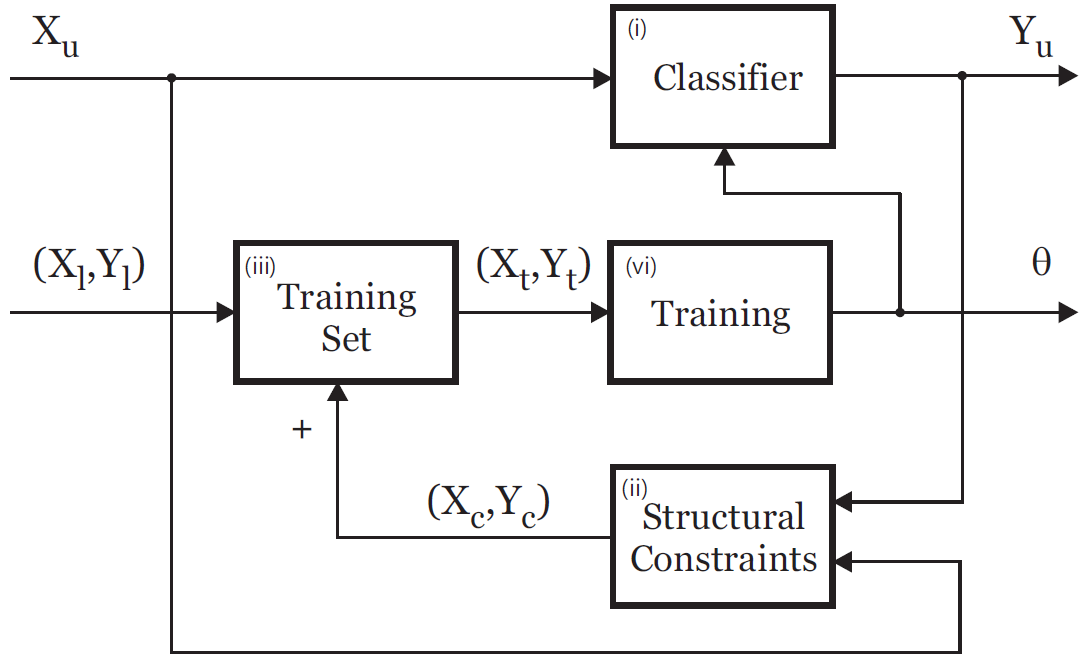
\includegraphics[scale=0.4]{../pictures/PN_LEARNING.png}\caption{Arbeitsweise P-N Learning (Quelle: \cite{PNL})}
	\label{PNL_Pic}
	\par\end{centering}
	\end{figure}

	\subsubsection{P-N Learning}

	\begin{comment}
	Im Wesentlichen besteht jeder Lernalgorithmus aus zwei Funktionen: Bewertungsfunktion und Lernfunktion. Die Bewertung übernimmt hier der Classfifier. Lernen wird durch P-N wird durch Constraints vorbereitet - sie generieren die positiven und negativen Beispiele, wobei hier die positiven am Wichtigsten sind.
	\end{comment}

	Sei $X$ ein Beispielraum (Feature-Space) und $x\in X$ ein Beispiel, und sei $Y=\{-1,1\}$ ein Labelraum und $y\in Y$ ein Label. Eine Menge von Beispielen $X$ und mit entsprechenden Labels $Y$ sei die markierte (gelabelte) Menge $(X,Y)$. Die Aufgabe von P-N Learning ist die Funktion $f:X\rightarrow Y$, parametrisiert mit $\Theta$, von einer initialen Menge $(X_{l},Y_{l})$ zu lernen und mittels ungelabelter Daten $X_{u}$ dessen Arbeitsweise zu verbessern. . $f$ ist somit ein Classifier, der mittels bootstrapping trainiert wird.

	\paragraph{Bootstrapping}
	Lernen das Klassifizierers durch Erweiterung des Trainingsets mittels Beispielen, die durch die Constraints aus den ungelabelten Daten gewonnen werden. Initialisierung durch bereits gelabelte (also positive und negative Beispiele). Von da an erfolgt die Abarbeitung iterativ.

	In Schritt $k$ hat der Klassifizierer bereits $k-1$ mal Labels zu unmarkierten Beispielen bestimmt, mit $y_{u}^{k}=f(x_{y}|\Theta^{k-1})$, wobei in jedem Schritt nur ein Beispiel berechnet wird. Die Constraints bewerten im Anschluss die erzeugte Ausgabe und prüfen, ob die Labels den erwarteten Bedingungen genügen. Sollte dies nicht der Fall sein, werden sie gegenfalls umgelabelt und werden der Trainingsmenge hinzugefügt. Ist dieser Schritt abgeschlossen, wird der Klassifizierer mit Hilfe der erweiterten Trainingsdaten trainiert und die Abarbeitung beginnt mit der nächsten Iteration $k+1$ von vorn.

	\paragraph{Constraints}
	Die Constraints dienen zum Bewerten der Detection-Ergebnisse und zur Generierung der Trainingsmenge. Die wichtigste Aufgabe besteht darin, nur solche Beispiele für die Lernprozedur zu filtern, die ``gut genug'' und gleichzeitig ``nicht zu gut'' sind. Dazu wird das Ergebnis des Trackers mit der Ergebnismenge des Detectors verglichen. Hat der Detector ein Objekt gefunden, das mit dem des Trackers übereinstimmt, wird nicht gelernt, da die verwendete Datenbasis des Classifiers anscheinend gut genug war. Findet der Tracker allerdings ein Objekt, das nicht mit der Ergebnismenge übereinstimmt, wird geschätzt, welches Ergebnis am plausibelsten ist. Dies geschieht auf Grundlage der vorhanden Datenbasis.

	Hier können zwei Fälle eintreten:
	\begin{enumerate}
	\item Das Ergebnis des Trackers ist ``besser'': In diesem Fall ist die gefundene Version des Objekts noch nicht in der Datenbasis und dient als Grundlage für ein positives Beispiel in der nächsten Lernphase.
	\item Das Ergebnis des Detectors ist ``besser'': Damit wurde das gesuchte Objekt gefunden und der Tracker hat anscheinend aus unterschiedlichen Gründen den Fokus verloren. Deshalb muss er reinitialisiert werden, und zwar auf das Objekt, das der Detector gefunden hat.
	\end{enumerate} 

	Ein Constraint ist in erster Linie eine Funktion, die als Parameter eine Menge von gelabelten Beispielen des Classifiers $(X_{u},Y_{u}^{k})$ erwartet und eine Menge von Beispielen $(X_{c}^{k},Y_{c}^{k})$, deren Label geändert wurden, als Ergebnis liefert. Die Anzahl dieser Constraints kann in diesem Fall beliebig sein, allerdings werden sie in zwei Kategorien geordnet: $P$ und $N$. 

	\textit{P-constraints} dienen zur Identifikation von Beispielen, die vom Classifier zwar als negativ bewertet, von den Constraints allerdings als positiv angesehen werden. \textit{N-constraints} hingegen identifizieren negative Beispiele, die vom Classifier fälschlicherweise als postitiv bewerten wurden. Dabei sind in der $k$-ten Itereration $n^{+}(k)$ die Anzahl der Beispiele, die ein neues postives Label und $n^{-}(k)$, die Anzahl der Beispiele, die durch die Constraints ein neues negatives Label erhalten haben. Dadurch werden zum einen neue postivie Beispiele erzeugt, die der Classifier noch nicht kennt und zusätzlich werden negative Beispiel generiert, die in der nächsten Iteration nicht fälschlicherweise als positiv bewertet werden. 

	\subsection{Zusammenspiel der Komponenten}
	Nachdem die einzelnen Teile des Tracking-Detection-Learning-Systems im Detail vorgestellt und behandelt wurden, erfolgt in diesem Abschnitt eine kurze Erläutering des Zusammenspiels aller Komponenten.

	\begin{figure}
	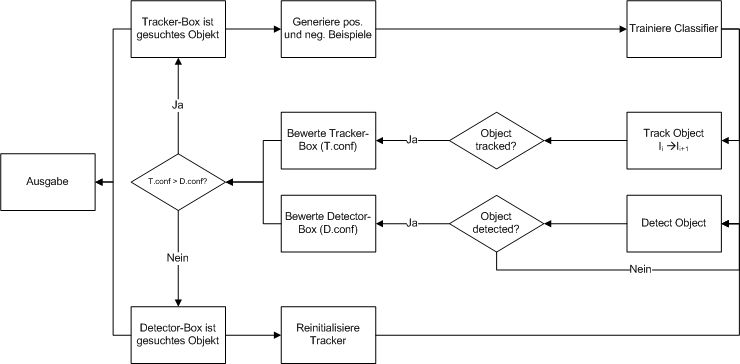
\includegraphics[scale=0.5]{../pictures/PAP.png}

	\caption{Zusammenspiel der Komponenten im Programmablaufplan}
	\end{figure}

	Prinzipiell ist für die Initalisierung von TLD eine Nutzereingabe erforderlich. Diese Dient einzig der Markierung des gesuchten Objekts. \label{subsection:working_components} Entweder wird in einem Ausgabebild das Objekt durch ein Rechteck markiert, oder ein bereits erzeugtes Model wird geladen, wordurch die Classifier mit den entsprechenden Datenbasen initialisiert werden. Ein dritte Möglichkeit biete eine vorgeschaltete Komponente, wie zum Beispiel ein alternativer Klassifizierer, der für die Erkennung eines bestimmten Objekts trainiert wird und die initialie BoundingBox liefert. Nachdem die Initialisierung durchgeführt wurde, arbeitet TLD selbständig und ohne weitere Eingaben von Außen. Die Tracking- sowie die Detection-Komponente arbeiten vollkommen unabhängig und parallel. Beide liefern nach der Abarbeitung ein Ergebnis in Form einer Box, die Kandidaten für das gesuchte Objekt sind. Aufgrund des Sliding-Window-Ansatzes und des abschließenden Clusterings ist es möglich, dass der Detector mehr als eine mögliche Box als Ausgabe bestimmt, also kein eindeutiges Ergebnis liefert. In diesem Fall wird für die folgende Bewertung nur die Box des Trackers berücksichtigt, und die Ergebnismenge des Detectors wird verworfen.

	Liefern Detector und Tracker jeweils eine Box, wird mittels NearestNeigbour-Classifier bestimmt, welche der beiden Boxen am Ehesten dem gesuchten Objekt entspricht. Die berechneten Werte sind $T.conf$ für den Confidense-Value des Trackerergebnisses beziehnungsweise $D.conf$ für den Confidense-Value des Detectorergebnisses.

	\paragraph{$T.conf\geq D.conf$}
	Die Box des Trackers hat einen höheren Confidense-Value als die des Detectors. Das bedeutet, dass die Classifier, die Teil des Detectors sind, das Objekt in seiner gefundenen Form nicht erkannt habe, was wiederum bedeutet, dass neue Beispiele generiert werden müssen. Der Trainingsprozess wird angestoßen, die synthetischen positiven Beispiele werden generiert und der Lernfunktion übergeben. Diese bewertet wiederum jedes Beispiel mittels des NearsestNeighbour-Classifier und wenn es ``zu gut'' ist, das heißt $conf\geq.65$, wird das Beispiel verworfen.

	\paragraph{$T.conf<D.conf$ }
	Der Detector liefert das bessere Ergebnis, was wiederum bedeutet,	dass der Tracker das Objekt nicht finden konnte, weil es verdeckt oder teilweise nicht sichtbar war, oder der Tracker gedrifftet ist. In jedem Fall wird der Tracker mit der Detector-Box reinitalisiert. Ein Training findet in diesem Fall nicht statt.

	\subsection{Initialisierung}
	Wie bereits in bei \ref{subsection:working_components} erwähnt, gibt es verschiedene Möglichkeiten TLD zu initialisieren. Einzig die Repräsentation des Objekts mittels BoundingBox mit gewährleistet sein. Da die Kopter sich automatische gegenseitig erkennen sollen und kein weiterer Objekt-Detector als TLD implementiert werden soll, wird initial ein bereits erzeugtes und trainiertes Modell eine Kopters geladen. Der Ablauf des Trainings wird in \ref{subsection:learning_and_testing} näher erläutert.